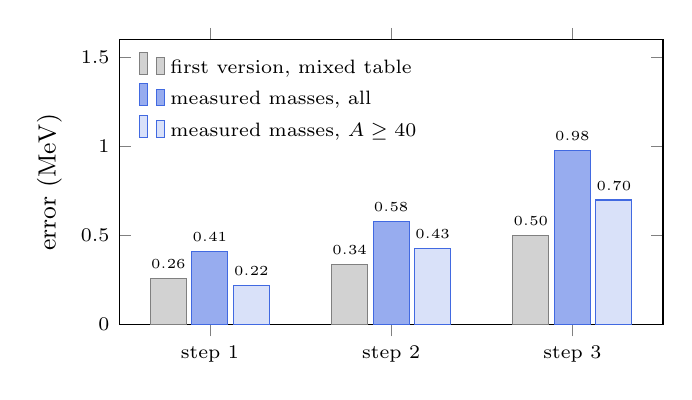
\begin{tikzpicture}
\begin{axis}[width=0.7\textwidth, height=5.2cm, ybar, bar width=13pt, ymin=0, ymax=1.6, ytick={0,0.5,1,1.5},
  symbolic x coords={step 1,step 2,step 3}, xtick=data, enlarge x limits=0.25, ylabel={error (MeV)},
  tick label style={font=\scriptsize}, label style={font=\small}, nodes near coords, nodes near coords style={font=\tiny, /pgf/number format/.cd, fixed, fixed zerofill, precision=2},
  legend style={font=\scriptsize, draw=none, at={(0.02,0.98)}, anchor=north west}, legend cell align=left, grid=none]
\addplot[fill=gray!35, draw=gray] coordinates {(step 1,0.26) (step 2,0.34) (step 3,0.50)};\addlegendentry{first version, mixed table}
\addplot[fill=RoyalBlue!55, draw=RoyalBlue] coordinates {(step 1,0.41) (step 2,0.58) (step 3,0.98)};\addlegendentry{measured masses, all}
\addplot[fill=RoyalBlue!20, draw=RoyalBlue] coordinates {(step 1,0.22) (step 2,0.43) (step 3,0.70)};\addlegendentry{measured masses, $A \ge 40$}
\end{axis}
\end{tikzpicture}
